\normaltrue \difficilefalse \tdifficilefalse
\correctiontrue

%\UPSTIidClasse{11} % 11 sup, 12 spé
%\newcommand{\UPSTIidClasse}{11}

\exer{Diagramme de Bode$\star$ \label{C2:02:510}}
\setcounter{numques}{0}
\UPSTIcompetence[2]{C2-02}
\index{Compétence C2-02}
\index{Diagramme de Bode}
\ifcorrection
\else
\textbf{Pas de corrigé pour cet exercice.}
\fi


\ifprof 
\else
 \fi
 
\question{Tracer le diagramme de Bode de la fonction de transfert suivante : $F_1(p)=\dfrac{15}{1+10p}$.}

\ifprof

\textbf{Tracer asymptotique}

\begin{center}
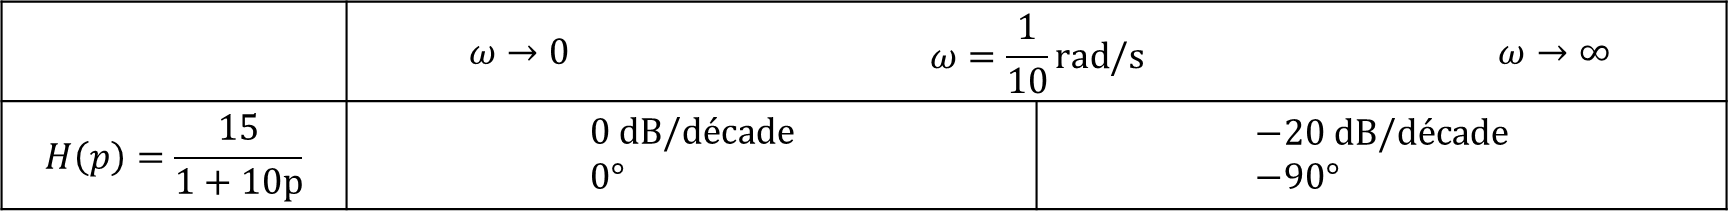
\includegraphics[width=.9\linewidth]{tab_01}
\end{center}


\begin{tikzpicture}[xscale=7/6]
\tikzset{
semilog lines/.style={thin, bleuxp}, 
semilog lines 2/.style={semilog lines,bleuxpc},
semilog half lines/.style={semilog lines 2,dotted },
semilog label x/.style={semilog lines,below,font=\tiny,black},
semilog label y/.style={semilog lines,right,font=\tiny,black}
}
\begin{scope}[yscale=3/50]
\semilog{-2}{2}{0}{30}

\BodeAmp[orangexp,thin,samples=100]{-2:2}{\POAmpAsymp{20}{0.2}}
\BodeAmp[orangexp,ultra thick]{-2:2}{\POAmp{20}{0.2}}
\draw (-1,28) node {\footnotesize $20\log K$, 0 dB/d\'ecade};
\draw (1.7,20) node {\footnotesize $-$20 dB/d\'ecade};
\draw [dashed,thick,bleuxp] (.7,0) -- (.7,25);
\draw (.7,0)  node {\Huge $\cdot$} node [above right]{\footnotesize $\dfrac{1}{\tau}$};
\end{scope}
\begin{scope}[yshift=-0.5cm,yscale=1/50]
\UniteDegre
\OrdBode{30}
\semilog{-2}{2}{-90}{0}
\BodeArg[orangexp,samples=100,thin]{-2:2}{\POArgAsymp{20}{0.2}}
\BodeArg[orangexp,ultra thick]{-2:2}{\POArg{20}{0.2}}
\end{scope}
\end{tikzpicture}


\textbf{Positionnement du diagramme de gain}
Lorsque que $\omega$ tend vers 0, le gain tend vers $20 \log 15 = \SI{23,5}{dB}$.


\begin{center}
 \begin{tikzpicture}[xscale=2]
\tikzset{
semilog lines/.style={thin, bleuxp}, 
semilog lines 2/.style={semilog lines,bleuxpc},
semilog half lines/.style={semilog lines 2,dotted },
semilog label x/.style={semilog lines,below,font=\tiny,black},
semilog label y/.style={semilog lines,right,font=\tiny,black}
}
\begin{scope}[yscale=1/20]
\semilog{-3}{1}{-30}{30}

\BodeAmp[orangexp,thin,samples=100]{-3:1}{\POAmpAsymp{15}{10}}
\BodeAmp[orangexp,ultra thick]{-3:1}{\POAmp{15}{10}}
\draw (-2.2,27) node {\footnotesize 23,5 dB, 0 dB/d\'ecade};
\draw (.3,15) node {\footnotesize $-$20 dB/d\'ecade};
\draw [dashed,ultra thick,bleuxp] (-1,-1) -- (-1,23.5);
\draw (-1,-1)  node {\Huge $\cdot$} node [above right]{\footnotesize 0,1};
\end{scope}
\begin{scope}[yshift=-3cm,yscale=1/90]
\UniteDegre
\OrdBode{45}
\semilog{-3}{1}{-180}{90}
\BodeArg[orangexp,samples=100,thin]{-3:1}{\POArgAsymp{15}{10}}
\BodeArg[orangexp,ultra thick]{-3:1}{\POArg{15}{10}}
\end{scope}
\end{tikzpicture}


%\begin{center}
%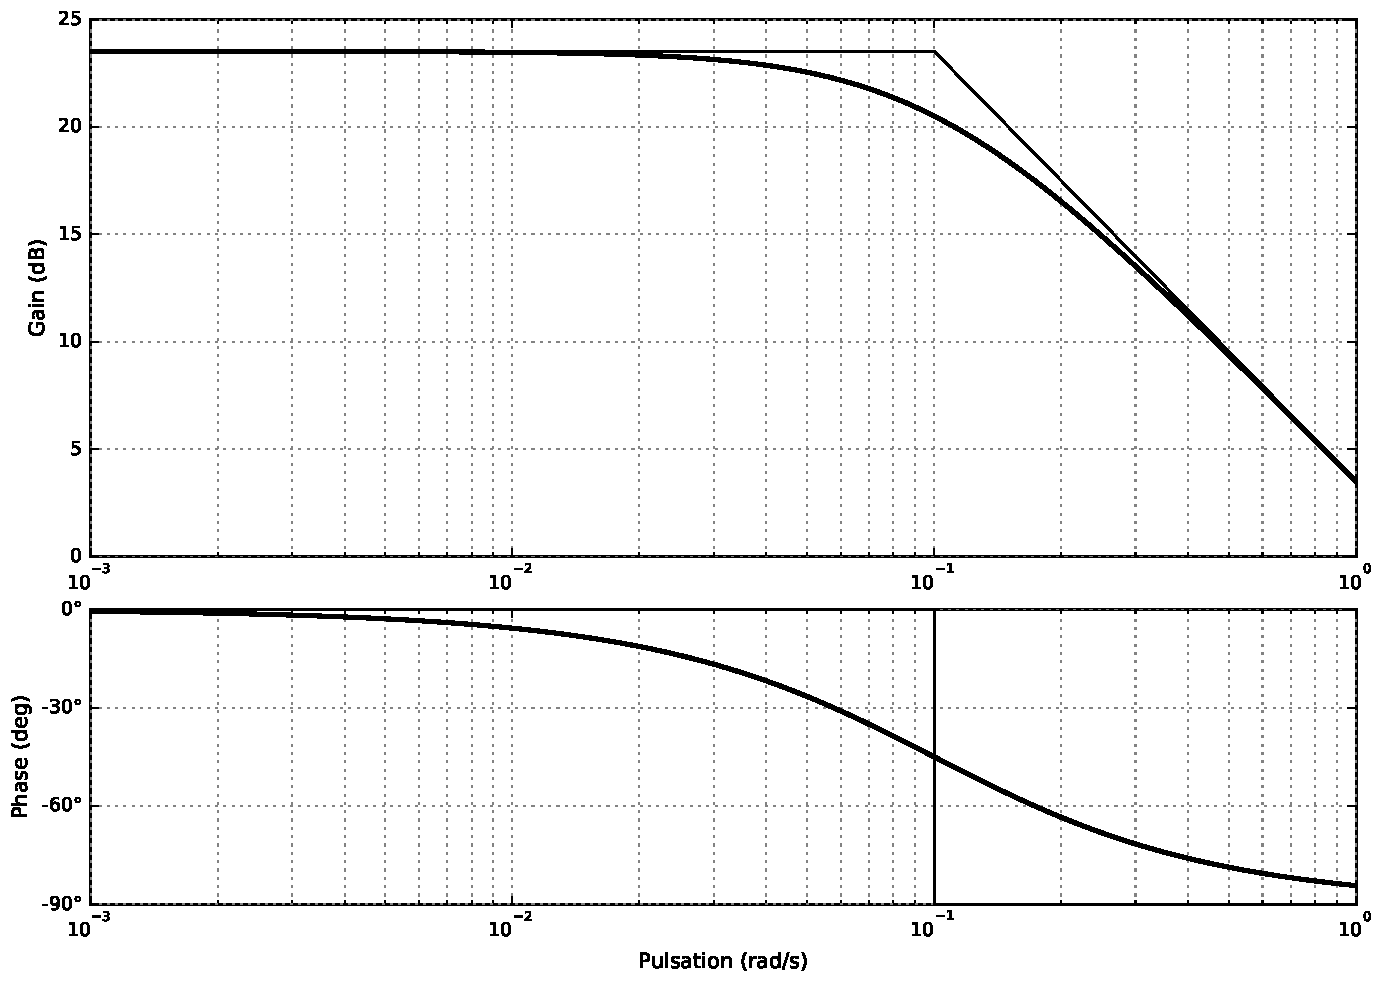
\includegraphics[width=.9\linewidth]{bode_01}
%\end{center}

\else 

\begin{center}
 \begin{tikzpicture}[xscale=2]
\tikzset{
semilog lines/.style={thin, bleuxp}, 
semilog lines 2/.style={semilog lines,bleuxpc},
semilog half lines/.style={semilog lines 2,dotted },
semilog label x/.style={semilog lines,below,font=\tiny,black},
semilog label y/.style={semilog lines,right,font=\tiny,black}
}
\begin{scope}[yscale=1/20]
\semilog{-3}{1}{-30}{30}

\end{scope}
\begin{scope}[yshift=-3cm,yscale=1/90]
\UniteDegre
\OrdBode{45}
\semilog{-3}{1}{-180}{90}

\end{scope}
\end{tikzpicture}

\fi


\question{Tracer le diagramme de Bode de la fonction de transfert suivante : $F_2(p)=\dfrac{10}{\left(1+10p\right)\left(10+p\right)}$.}
\ifprof
\textbf{Tracer asymptotique}

$F_2(p)=\dfrac{1}{\left(1+10p\right)\left(1+\dfrac{p}{10}\right)}$

\begin{center}
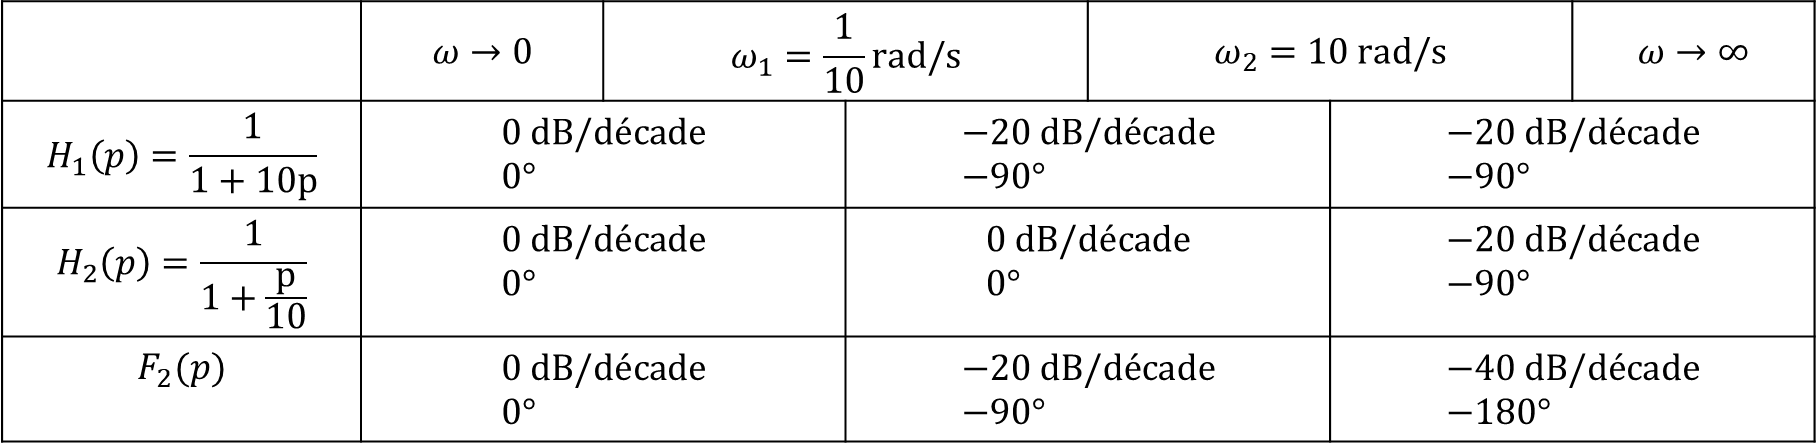
\includegraphics[width=.9\linewidth]{tab_02}
\end{center}


\textbf{Positionnement du diagramme de gain}
Lorsque que $\omega$ tend vers 0, le gain tend vers $20 \log 1 = \SI{0}{dB}$.


\begin{center}
 \begin{tikzpicture}[xscale=1.5]
\tikzset{
semilog lines/.style={thin, bleuxp}, 
semilog lines 2/.style={semilog lines,bleuxpc},
semilog half lines/.style={semilog lines 2,dotted },
semilog label x/.style={semilog lines,below,font=\tiny,black},
semilog label y/.style={semilog lines,right,font=\tiny,black}
}
\begin{scope}[yscale=1/40]
\semilog{-3}{3}{-140}{20}
\UnitedB
\OrdBode{20}
\BodeAmp[orangexp,thin,samples=101]{-3:3}{\POAmpAsymp{1}{10} + \POAmpAsymp{1}{10}}
\BodeAmp[orangexp,ultra thick]{-3:3}{\POAmp{1}{10} + \POAmp{1}{0.1}}

%\draw (-2.2,27) node {\footnotesize 23,5 dB, 0 dB/d\'ecade};
%\draw (.3,15) node {\footnotesize $-$20 dB/d\'ecade};
%\draw [dashed,ultra thick,bleuxp] (-1,-1) -- (-1,23.5);
%\draw (-1,-1)  node {\Huge $\cdot$} node [above right]{\footnotesize 0,1};
\end{scope}

\begin{scope}[yshift=-5cm,yscale=1/90]
\UniteDegre
\OrdBode{45}
\semilog{-3}{3}{-180}{90}
\BodeArg[orangexp,samples=101,thin]{-3:3}{\POArgAsymp{1}{10} + \POArgAsymp{1}{0.1}}
\BodeArg[orangexp,ultra thick]{-3:3}{\POArg{1}{10} + \POArg{1}{0.1}}
\end{scope}
\end{tikzpicture}
\end{center}
%
%\begin{center}
%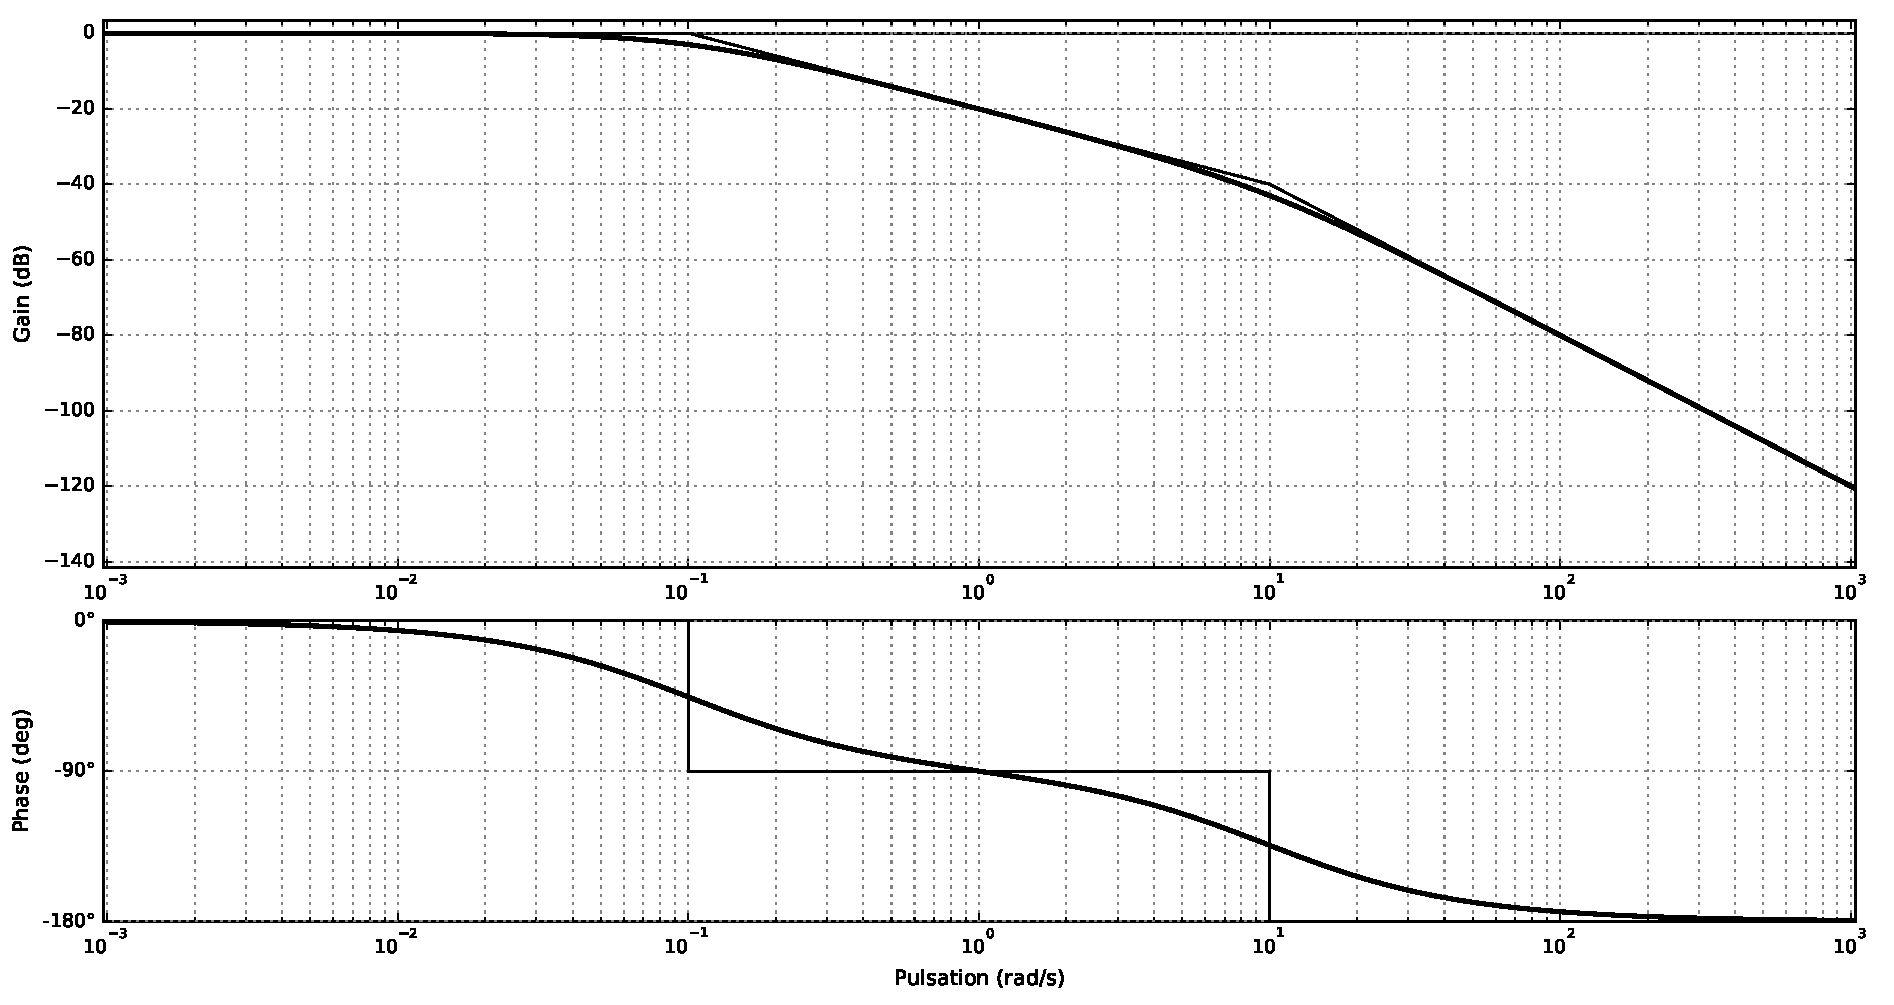
\includegraphics[width=.9\linewidth]{bode_02}
%\end{center}

\else 
%\begin{center}
%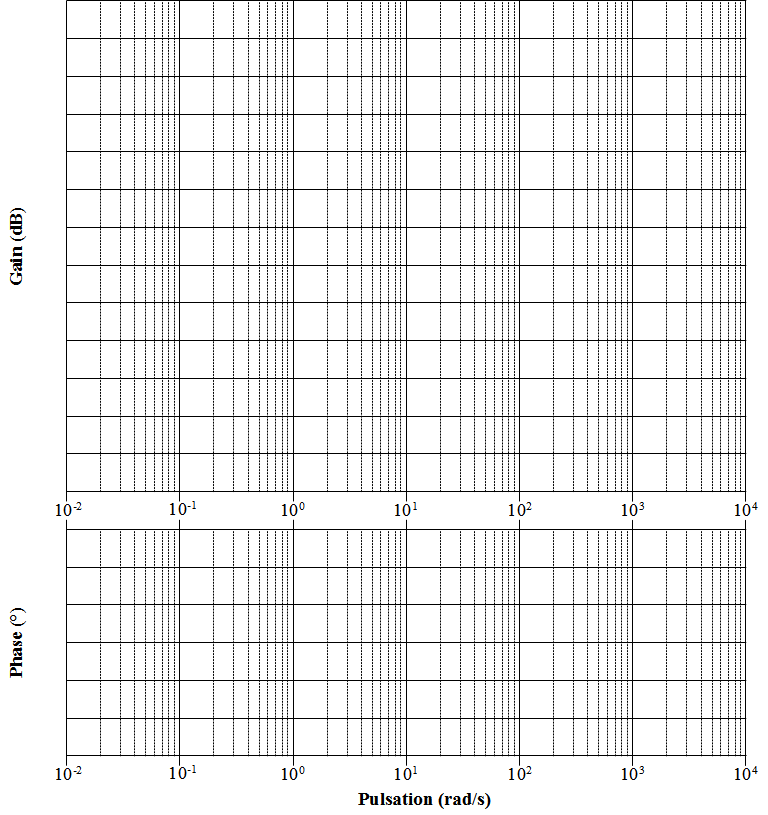
\includegraphics[width=.9\linewidth]{510_01}
%\end{center}
\begin{center}
 \begin{tikzpicture}[xscale=1.5]
\tikzset{
semilog lines/.style={thin, bleuxp}, 
semilog lines 2/.style={semilog lines,bleuxpc},
semilog half lines/.style={semilog lines 2,dotted },
semilog label x/.style={semilog lines,below,font=\tiny,black},
semilog label y/.style={semilog lines,right,font=\tiny,black}
}
\begin{scope}[yscale=1/40]
\semilog{-3}{3}{-140}{20}
\UnitedB
\OrdBode{20}

\end{scope}

\begin{scope}[yshift=-5cm,yscale=1/90]
\UniteDegre
\OrdBode{45}
\semilog{-3}{3}{-180}{90}

\end{scope}
\end{tikzpicture}
\end{center}


\fi


\question{Tracer le diagramme de Bode de la fonction de transfert suivante : $F_3(p)=\dfrac{40}{p\left(1+300p\right)}$.}
\ifprof

\textbf{Tracer asymptotique}

\begin{center}
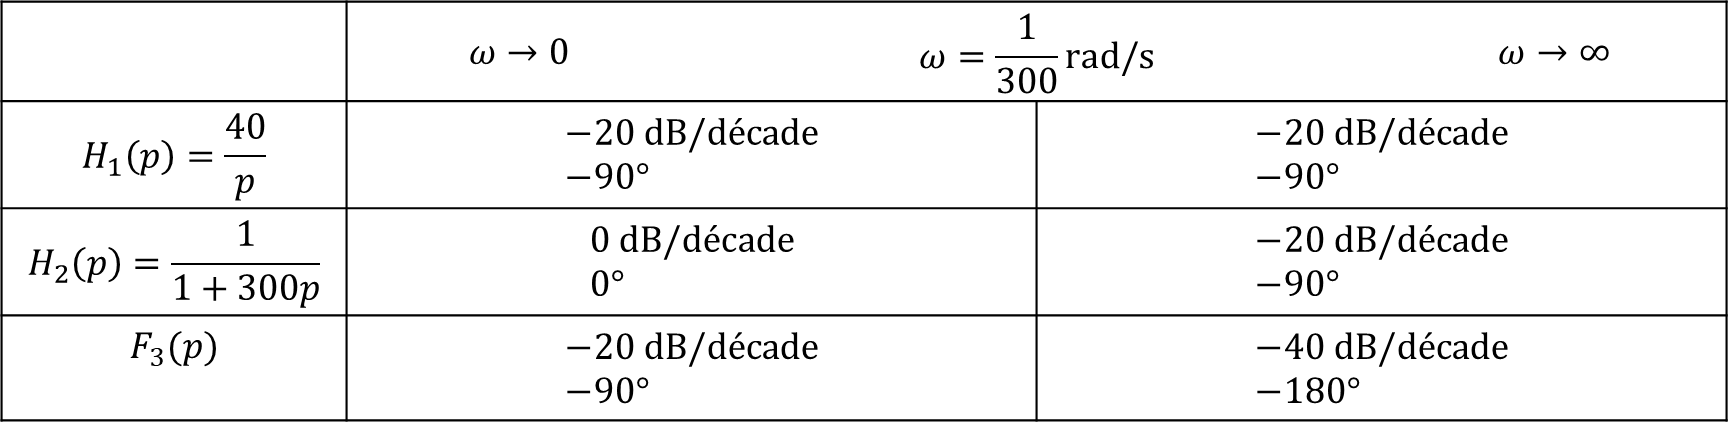
\includegraphics[width=.9\linewidth]{tab_03}
\end{center}


\textbf{Positionnement du diagramme de gain}
Lorsque que $\omega$ tend vers 0, $F_3(p)\simeq \dfrac{40}{p}$. Cette asymptote de pente \SI{-20}{dB/decade} passe par le point $(40,0)$. 

\begin{center}
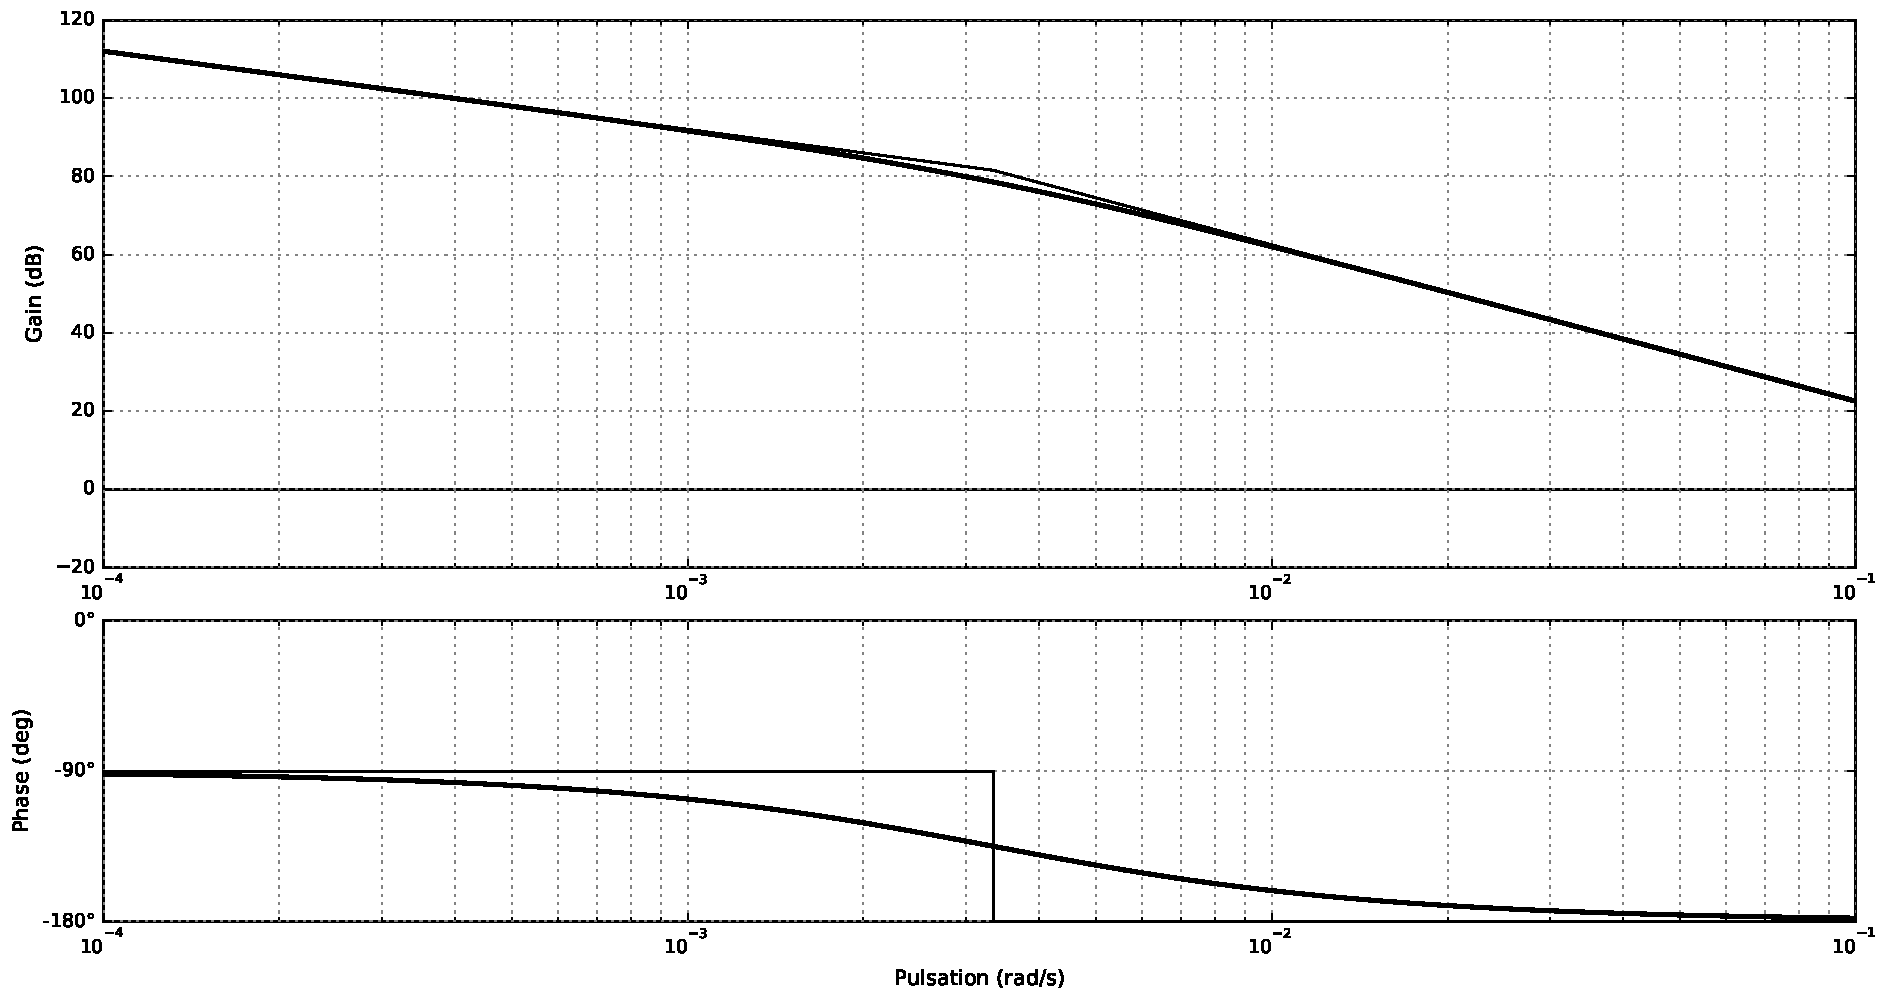
\includegraphics[width=.9\linewidth]{bode_03}
\end{center}

\else 
\begin{center}
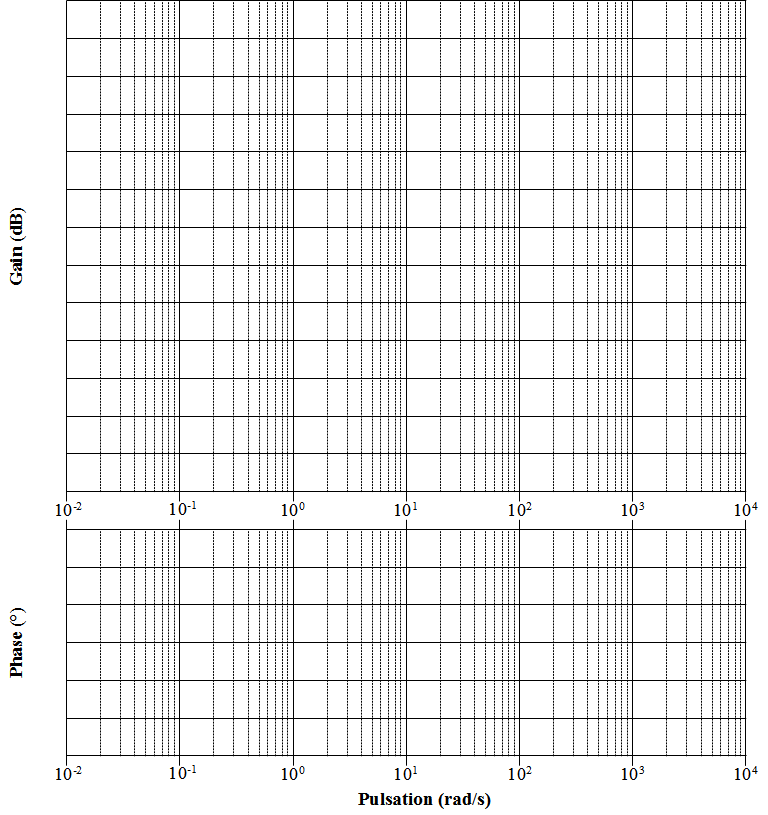
\includegraphics[width=.9\linewidth]{510_01}
\end{center}
\fi





%\question{Réaliser le schéma-blocs.}
%\ifprof
%\begin{figure}[H]
%\centering
%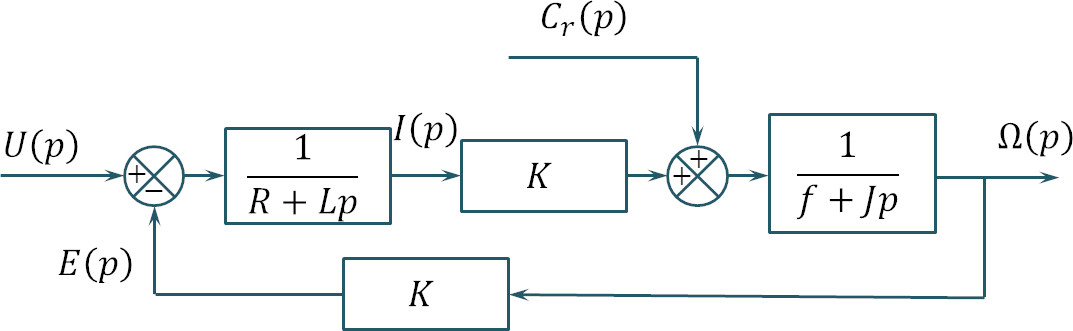
\includegraphics[width=\linewidth]{51_01_c}
%%\caption{Évolution du couple utile en fonction de la vitesse de rotation pour des
%%fréquences de commande de \SI{90}{Hz} à \SI{110}{Hz}. \label{fig_50_04}}
%\end{figure}
%\else
%\fi


\end{center}


\ifprof
\else
\begin{flushright}
\footnotesize{Corrigé  voir \ref{C2:02:510}.}
\end{flushright}%
\fi